\chapter{Theory}

\section{Image processing}
In the original drain tank system, regular water where used to fill the tank. Since water is a colourless liquid, it can be difficult to detect the water level in the tank with a RGB camera. To make this task easier, a colour was added to the water. After adding a blue colour to the water it would be easy to detect the water compared to the white background. 

\subsection{Saturation plane}
Since the water contains a blue that is quite "colourful" or with high saturation, the water can be detected by using the saturation plane in the "Hue, Saturation, Luminosity" model \textbf{(HSL)}. A 100 \% blue colour will be displayed as white in the saturation plane. The water in the drain tank has a very saturated blue colour. The tank rig itself and the background has rather low saturation (white, black and grey). The result of will be a almost black image where the blue water will be displayed as white.



\begin{figure}[t]
	\centering
	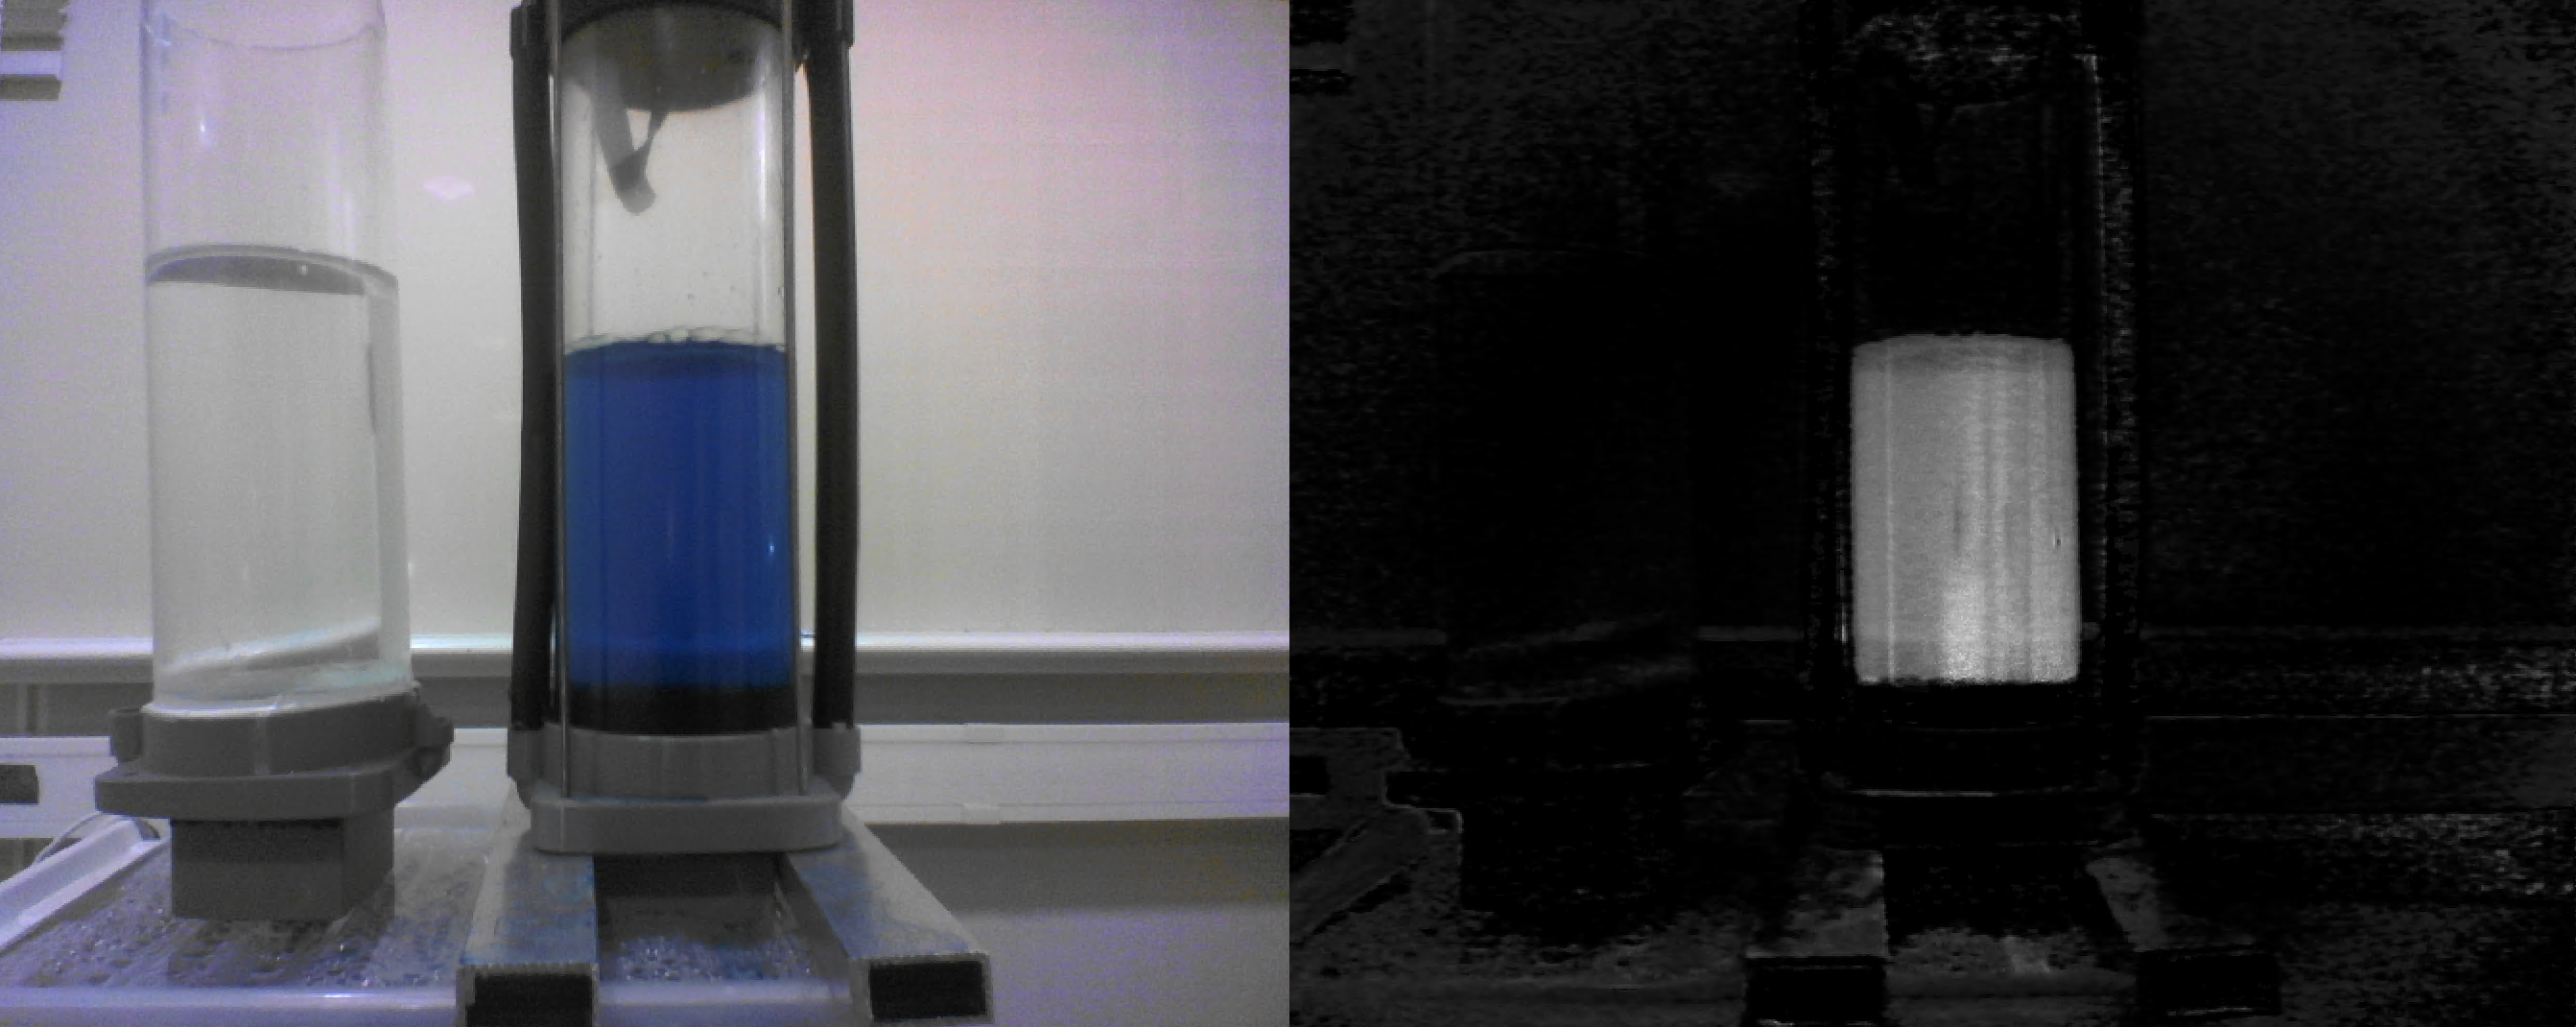
\includegraphics[width=1\textwidth]{pictures/SatRGB}
	\caption{Compearison between raw image (Left) and Saturation plane (Right)}
	\label{img:SRGB}
\end{figure}


As seen in \textbf{Figure \ref{img:SRGB}} The tank containing regular colourless water is almost invisible in the saturation plane while the blue water has become white.

\subsection{Filtering}
By using Fast Fourier Transform \textbf{(FFT)}, the grayscale image is converted into its frequency domain. In the frequency domain of the image, details and sharp edges are recognized as mid to high frequencies. By adding a low pass truncation filter with truncation frequency to 6.00 \%, the unwanted pars of the image becomes filtered out and leaves the blue water alone and easier to detect. The result of the FFT low pass filter are shown in \textbf{Figure \ref{img:FFTS}}.

\begin{comment}
    https://zone.ni.com/reference/en-XX/help/370281M-01/nivisionlvbasics/improve_an_image/ 
\end{comment}

\begin{figure}[b!]
	\centering
	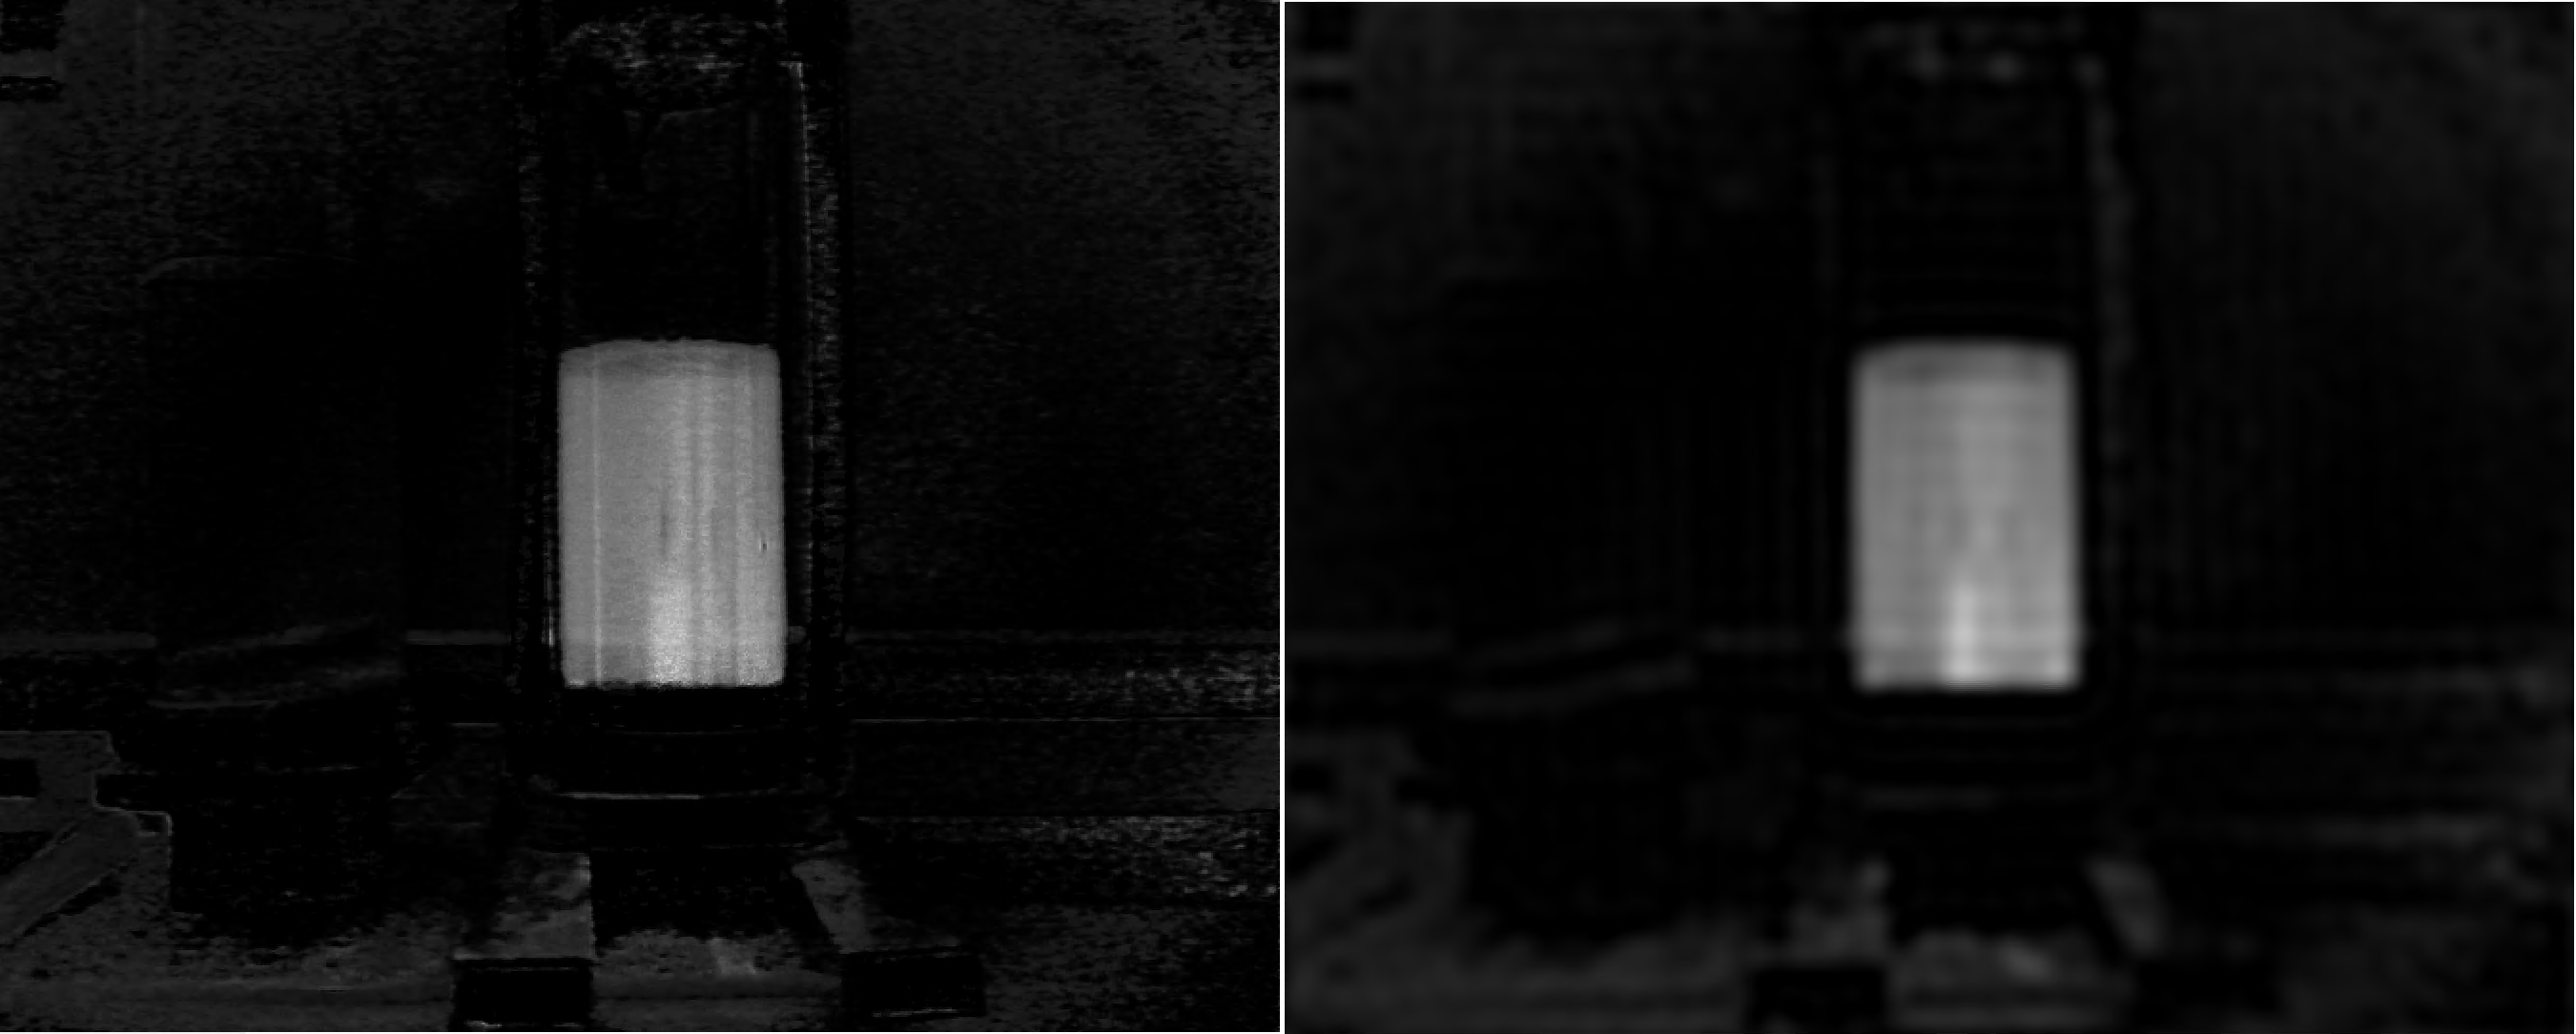
\includegraphics[width=1\textwidth]{pictures/FFTS}
	\caption{Compearison between unfiltered image (Left) and FFT filtered (Right)}
	\label{img:FFTS}
\end{figure}


\subsection{Creating a Binary Image}
The filtered grayscale image starting to become something that is useful to measure the water level with, but there is still some unwanted data in the image. To remove this the image is converted to a binary image by using threshold detection. Since the blue water in the grayscale image is white, the threshold detection was set to look for bright objects. When converting the image to a binary image is the values below 80 in the range 0-255 (0 \% - 100 \%) set to binary 0 and abowe 80 set to binary 1. With this threshold the binary image will be converted to a image with only two values of data in every pixels (\textbf{Figure \ref{img:BIN}}).



\begin{figure}[t!]
	\centering
	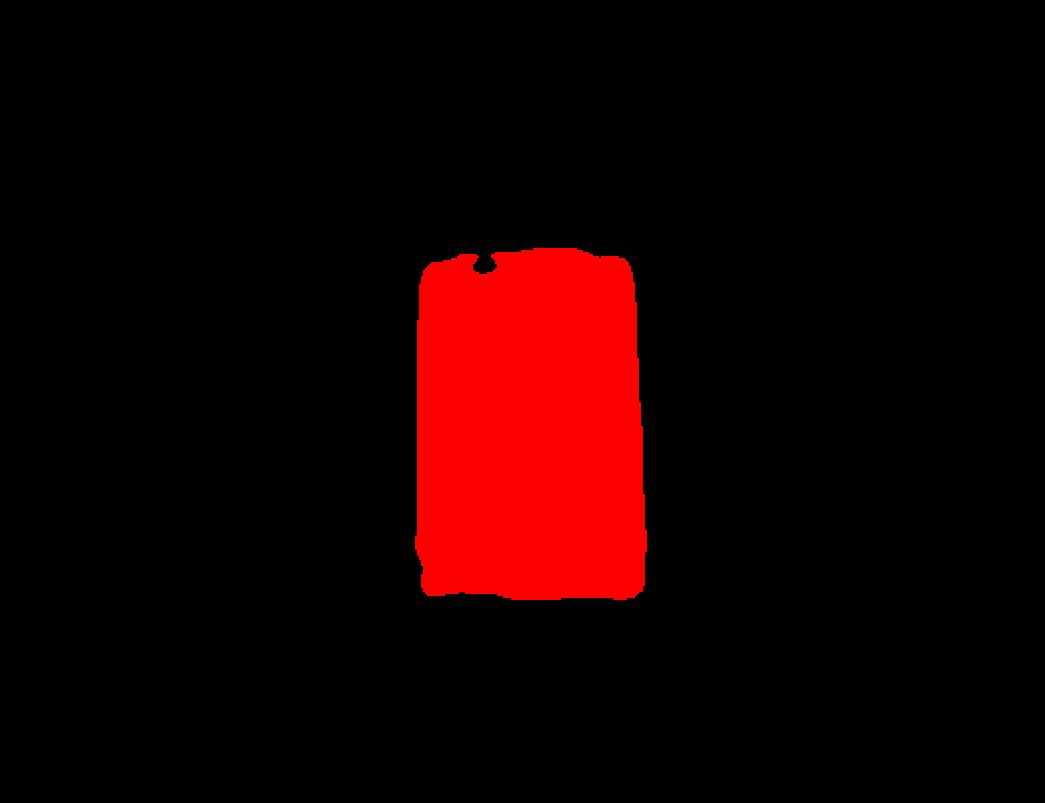
\includegraphics[width=0.75\textwidth]{pictures/BIN}
	\caption{Binary image of the blue water in the drain tank}
	\label{img:BIN}
\end{figure}